\documentclass[conference]{IEEEtran}
% \IEEEoverridecommandlockouts
% The preceding line is only needed to identify funding in the first footnote. If that is unneeded, please comment it out.
\usepackage{cite}
\usepackage{csquotes}
\usepackage{amsmath,amssymb,amsfonts}
\usepackage{algorithmic}
\usepackage{booktabs}
\usepackage{graphicx}
\usepackage{textcomp}
\usepackage{xcolor}
\usepackage{makecell}
\usepackage{float}
\usepackage{placeins}
\usepackage{hyperref}
\usepackage{tcolorbox}
\usepackage{tabularx}
\def\BibTeX{{\rm B\kern-.05em{\sc i\kern-.025em b}\kern-.08em
    T\kern-.1667em\lower.7ex\hbox{E}\kern-.125emX}}

\newcolumntype{P}[1]{>{\centering\arraybackslash}m{#1}}

\graphicspath{{./images/}}

\begin{document}

\title{Real-Time Road Sign Detection and Classification\\
}

\author{\IEEEauthorblockN{1\textsuperscript{st} Dumitru Mițca}
\IEEEauthorblockA{\textit{dept. CTI} \\
\textit{Technical University "Gheorge Asachi" of Iași}\\
Iași, Romania \\
dumitru.mitca@student.tuiasi.ro}
\and
\IEEEauthorblockN{2\textsuperscript{nd} Mihai Mihalache}
\IEEEauthorblockA{\textit{dept. CTI} \\
\textit{Technical University "Gheorge Asachi" of Iași}\\
Iași, Romania \\
mihai.mihalache2@student.tuiasi.ro}
\and
\IEEEauthorblockN{3\textsuperscript{rd} Otilia Zvorișteanu}
\IEEEauthorblockA{\textit{dept. CTI} \\
\textit{Technical University "Gheorge Asachi" of Iași}\\
Iași, Romania \\
otilia.zvoristeanu2@academic.tuiasi.ro}
\and
\IEEEauthorblockN{4\textsuperscript{th} Simona Caraiman}
\IEEEauthorblockA{\textit{dept. CTI} \\
\textit{Technical University "Gheorge Asachi" of Iași}\\
Iași, Romania \\
simona.caraiman@academic.tuiasi.ro}
}

\maketitle

\begin{abstract}
Road signs are a vital part of traffic infrastructure and their correct detection and classification
is a vital task in autonomous driving applications. In this paper, we present a cursory study over
state-of-the-art software solutions and related papers in the field, and then we present our initial
implementation of such an application.
\end{abstract}

\begin{IEEEkeywords}
computer vision, road sign detection, autonomous driving
\end{IEEEkeywords}

\section{Introduction}
Road sign detection and classification is a significant task in the computer vision space, that
has been studied for at least a decade and a half. Applications in this domain have strict requirements,
as mistakes or software bugs can lead to significant financial loss or even human death in the worst case,
requirements such as:
\begin{itemize}
    \item low, tending towards 0\%, misclassification rate --- classifying a stop sign as a right-of-way
    sign can lead to accidents, this example is unlikely to happen in a real application, but it shows
    the worst case scenario; more likely missclassication would be "must go left" as "must go right", or
    misclassifying the various "road thins ahead" signs between each other
    \item high speed --- a vehicle should not stop at every road sign it encounters in order to recognize it
    then proceed, abiding its instructions, this process should be real-time
    \item high tolerance to bad weather conditions --- fog, rain and snow are very common conditions in
    various parts of the world, an autonomous vehicle should be able to function correctly in any of these
    conditions. This point ties into the low missclassification rate point
    \item high tolerance to bad lightning --- similar to the above
    \item low hardware cost --- cars are already expensive, by including expensive high resolution cameras
    or expensive processors to run the detection and classification steps, the costs would be very unreasonable
    for the vast majority of people
\end{itemize}

\begin{figure}
    \centerline{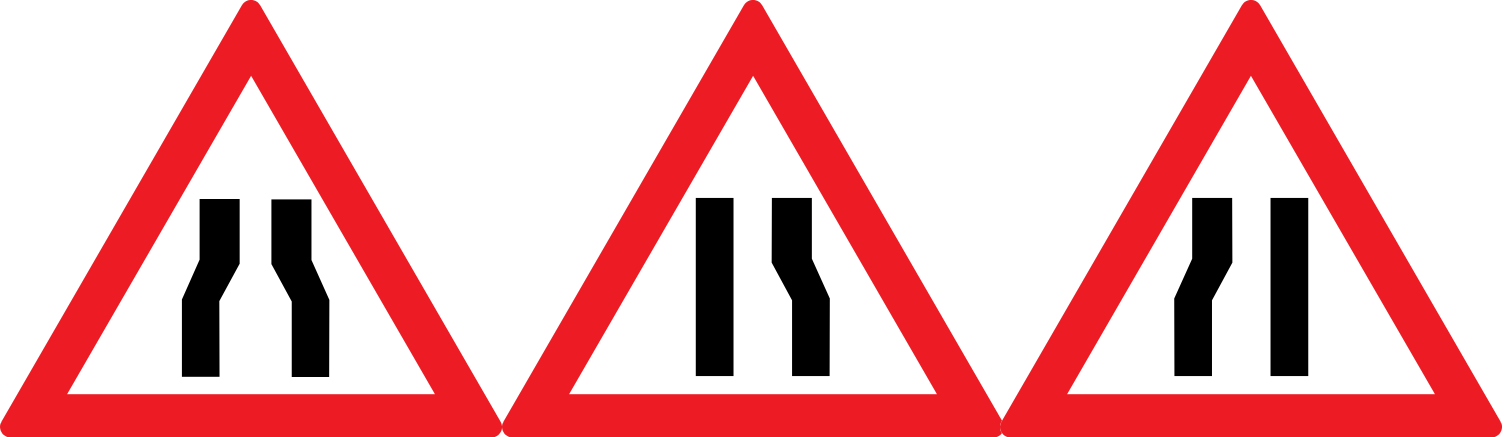
\includegraphics[width=\linewidth]{confusables}}
    \caption{Three confusable signs, in order from left to right: "Îngustarea șoselei din ambele sensuri",
    "Îngustarea șoselei din dreapta", "Îngustarea șoselei din stânga"\protect\footnotemark}
\end{figure}

\footnotetext{By Gigillo83, own work CC BY-SA 4.0, \url{https://commons.wikimedia.org/w/index.php?curid=40362644},
\url{https://commons.wikimedia.org/w/index.php?curid=40362647}, \url{https://commons.wikimedia.org/w/index.php?curid=40362645},
stitched by Mițca Dumitru into a single image under the same terms.}

\subsection{Related work}
We've surveyed a number of papers in this domain in order to discover what approach we should follow in our
own application.

Reference \cite{4370763} was interesting to read but ultimately we found the approach in this paper
to be limiting as it could only detect road signs with red borders that were either circles or triangles.

Reference \cite{Karthika2022} proposed an approach that had multiple layers of preprocessing before
the detection and classification itself, which was done using the YOLO (You only look once) architecture.

Reference \cite{metastudy2019}, a metastudy on the state of computer vision in traffic sign detection and
recognition in 2019, was very useful as it showed us approaches that would be likely be useful
with good accuracy and clear paths to take in development. It confirmed to us that an approach where
the detection and recognition steps were split was a good idea as it is what most of the literature
surveyed did. We initially believed that we could use grayscale datasets to simplify our machine learning
(ML) models, but \cite{metastudy2019} infirmed this belief showing us that colour-based approaches would
have higher accuracy. Reference \cite{4290244} claims that a grayscale approach would be based on shape
detection and be computationally expensive.

We approached \cite{8709983} due to its generic title, but it is an application in traffic sign inventory
management, and as such has less strict requirements than our application, and a much higher error rate
is acceptable in its domain.

Reference \cite{6196571} presents an approach where the detection of road signs is done using classical
segmentation methods, while the recognition itself is done using a multilayer perceptron neural network.

Reference \cite{svm_paper} presents an approach based on HOG\footnote{Histogram of Oriented Gradients}
features and linear support vector machines\footnote{See \hyperlink{appendixa}{Appendix A} for a summary on SVMs}
(SVMs). The paper proposes an approach where the HOG and SVM -based step is used for traffic sign detection and
a convolutional neural network is used for classification. Our final approach is similar to the one proposed by this paper.

Conclusions:
\begin{itemize}
    \item this kind of application should be split in two separate modules: a detection module and a
    recognition module, with any number of pre-processing before them
    \item the detection module can be implemented using classical methods, while the recognition
    module must be implemented using neural networks
    \item grayscale approaches are not computationally viable
\end{itemize}

\subsection{State of the art}

For existing software solutions we surveyed the pretrained YOLOv8\cite{Jocher_YOLO_by_Ultralytics_2023}\footnote{You Only Look Once}
model YOLOv8n and Roboflow.

\subsubsection{YOLOv8}
Through experimentation using the pretrained YOLOv8 model, we came to the conclusion that pretrained
models are unlikely to be useful to particular applications, due to the pretrained models' generality
and datasets where weather and or lightning conditions aren't varied enough. We believe using similar,
or the same, architectures used by pretrained models or fine-tuning them is a good path forward however.

\begin{figure}[h!]
    \centerline{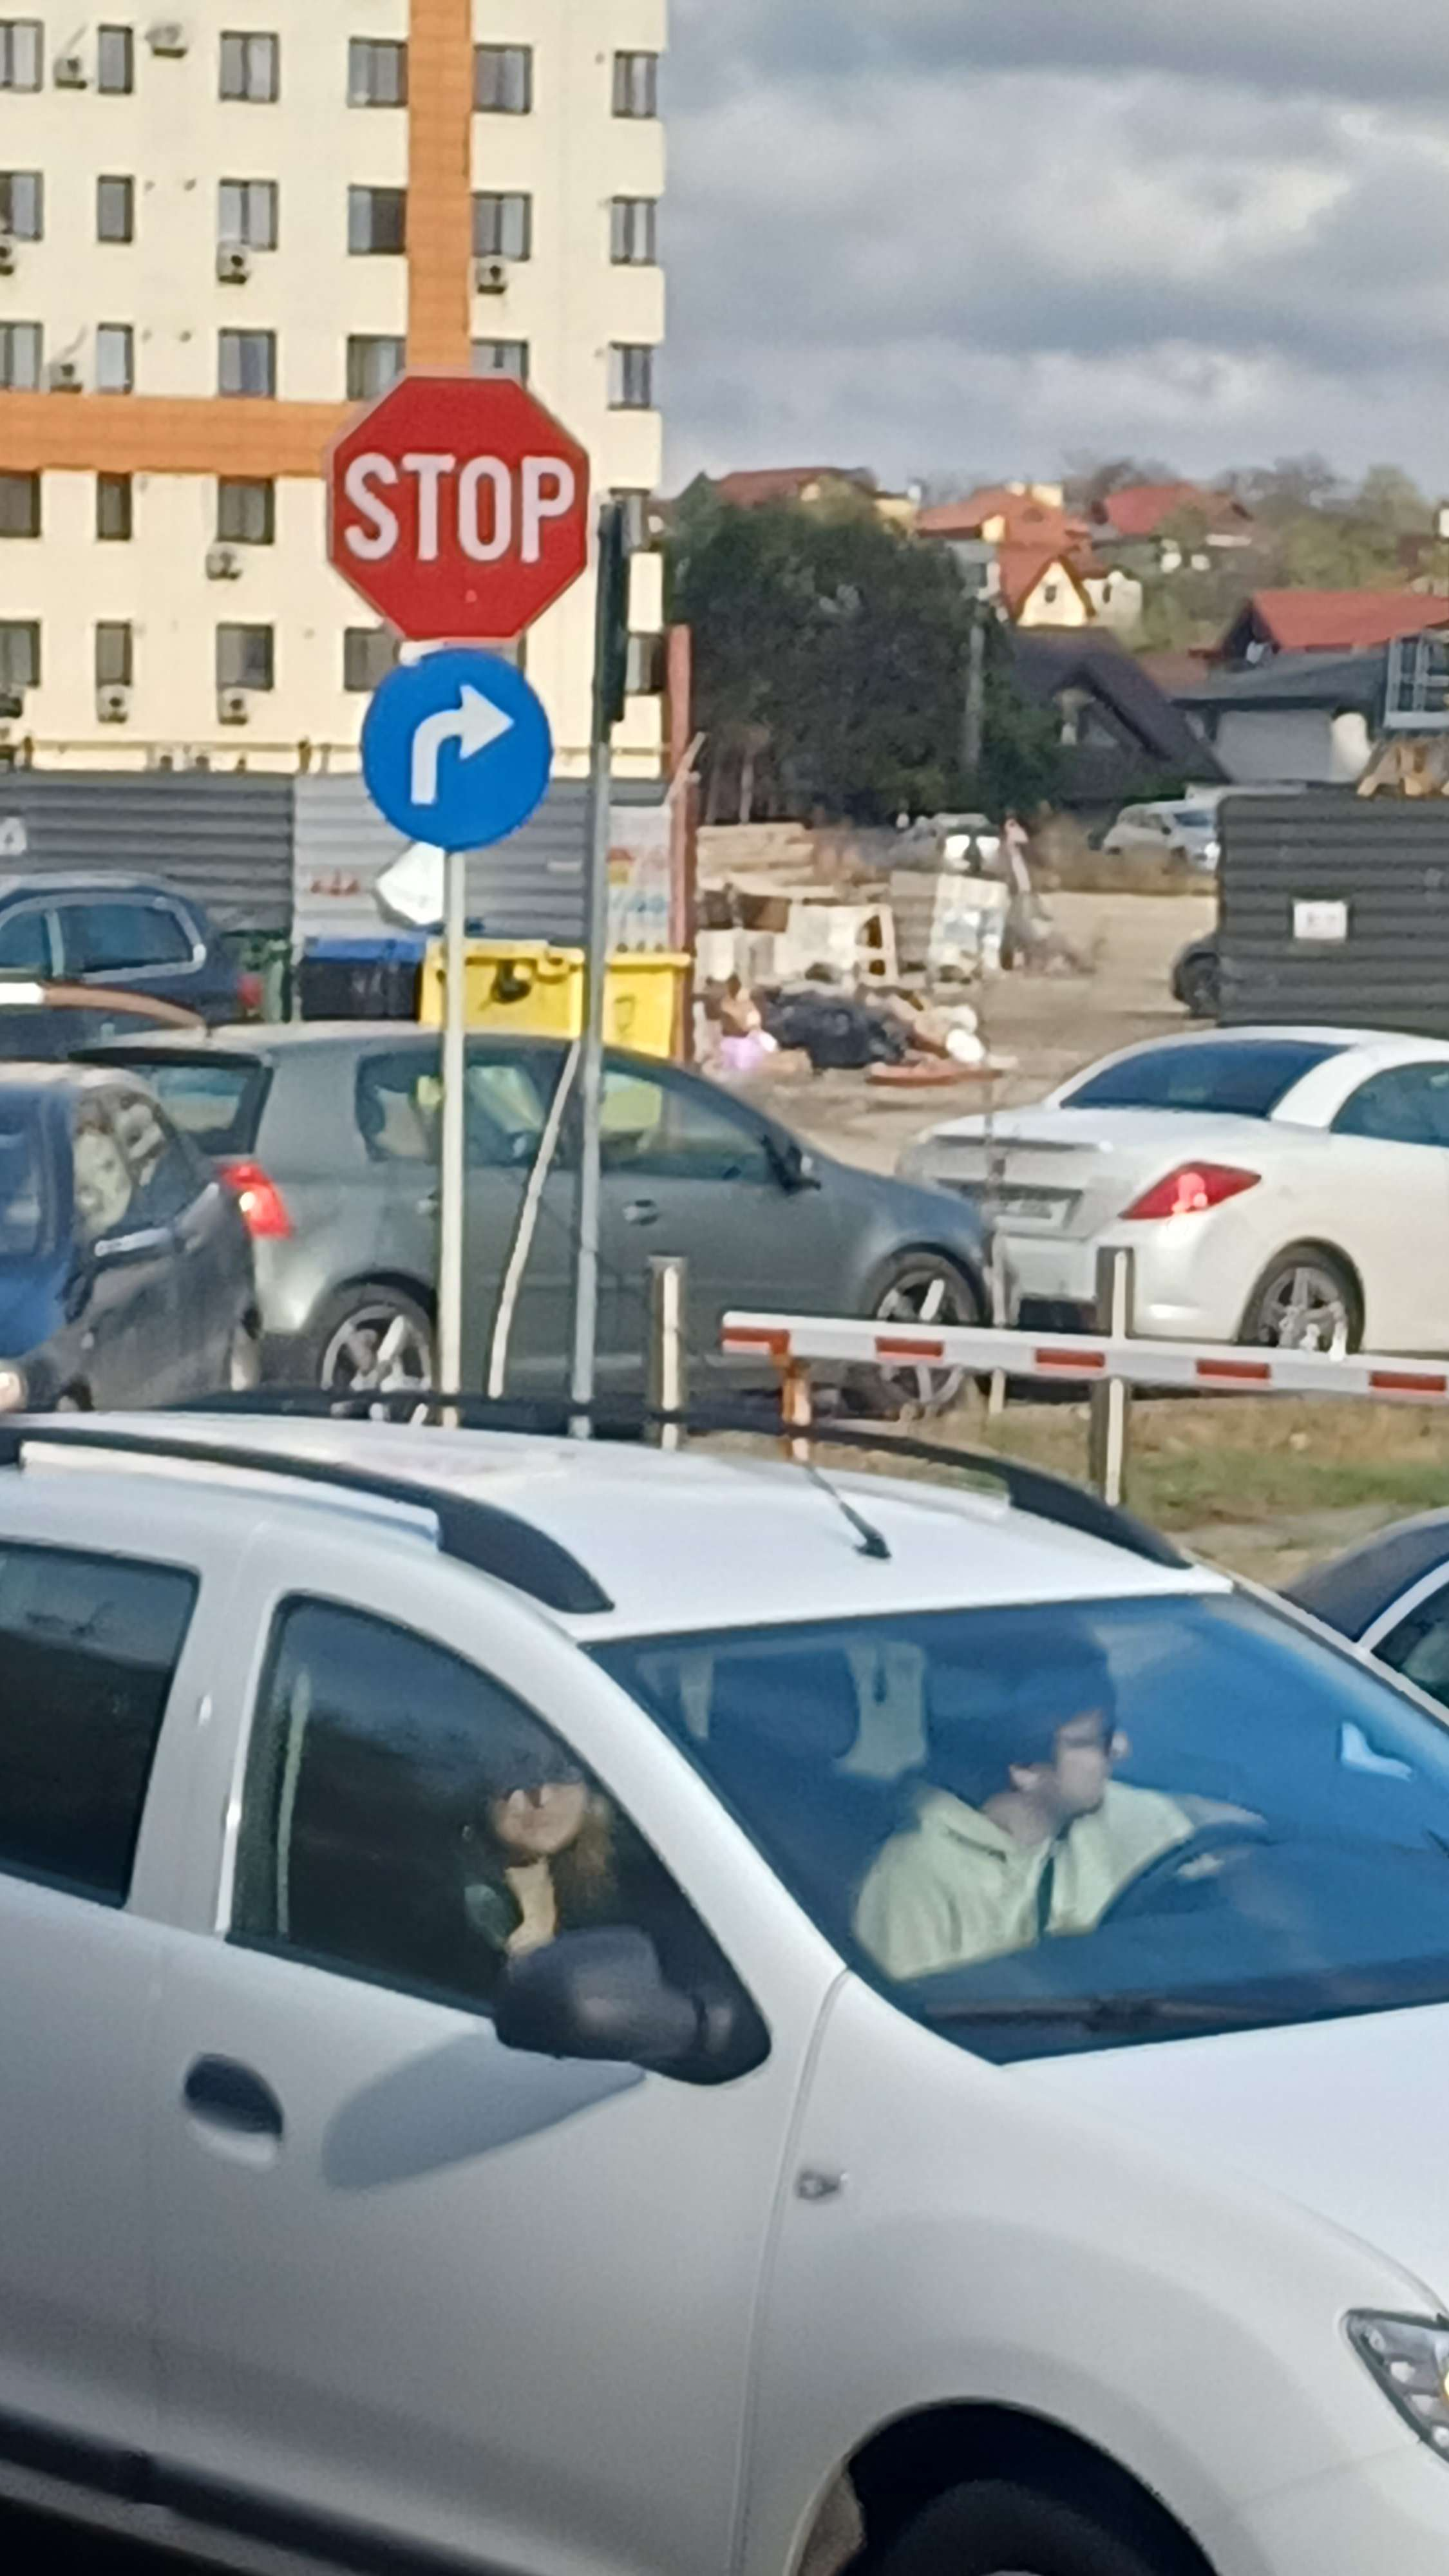
\includegraphics[width=0.5\linewidth,]{poza-fata-ac}}
    \caption{YOLOv8n with no additional training detects 2 stop signs in this image}
    \label{poza-fata-ac}
\end{figure}


\begin{figure}
    \centerline{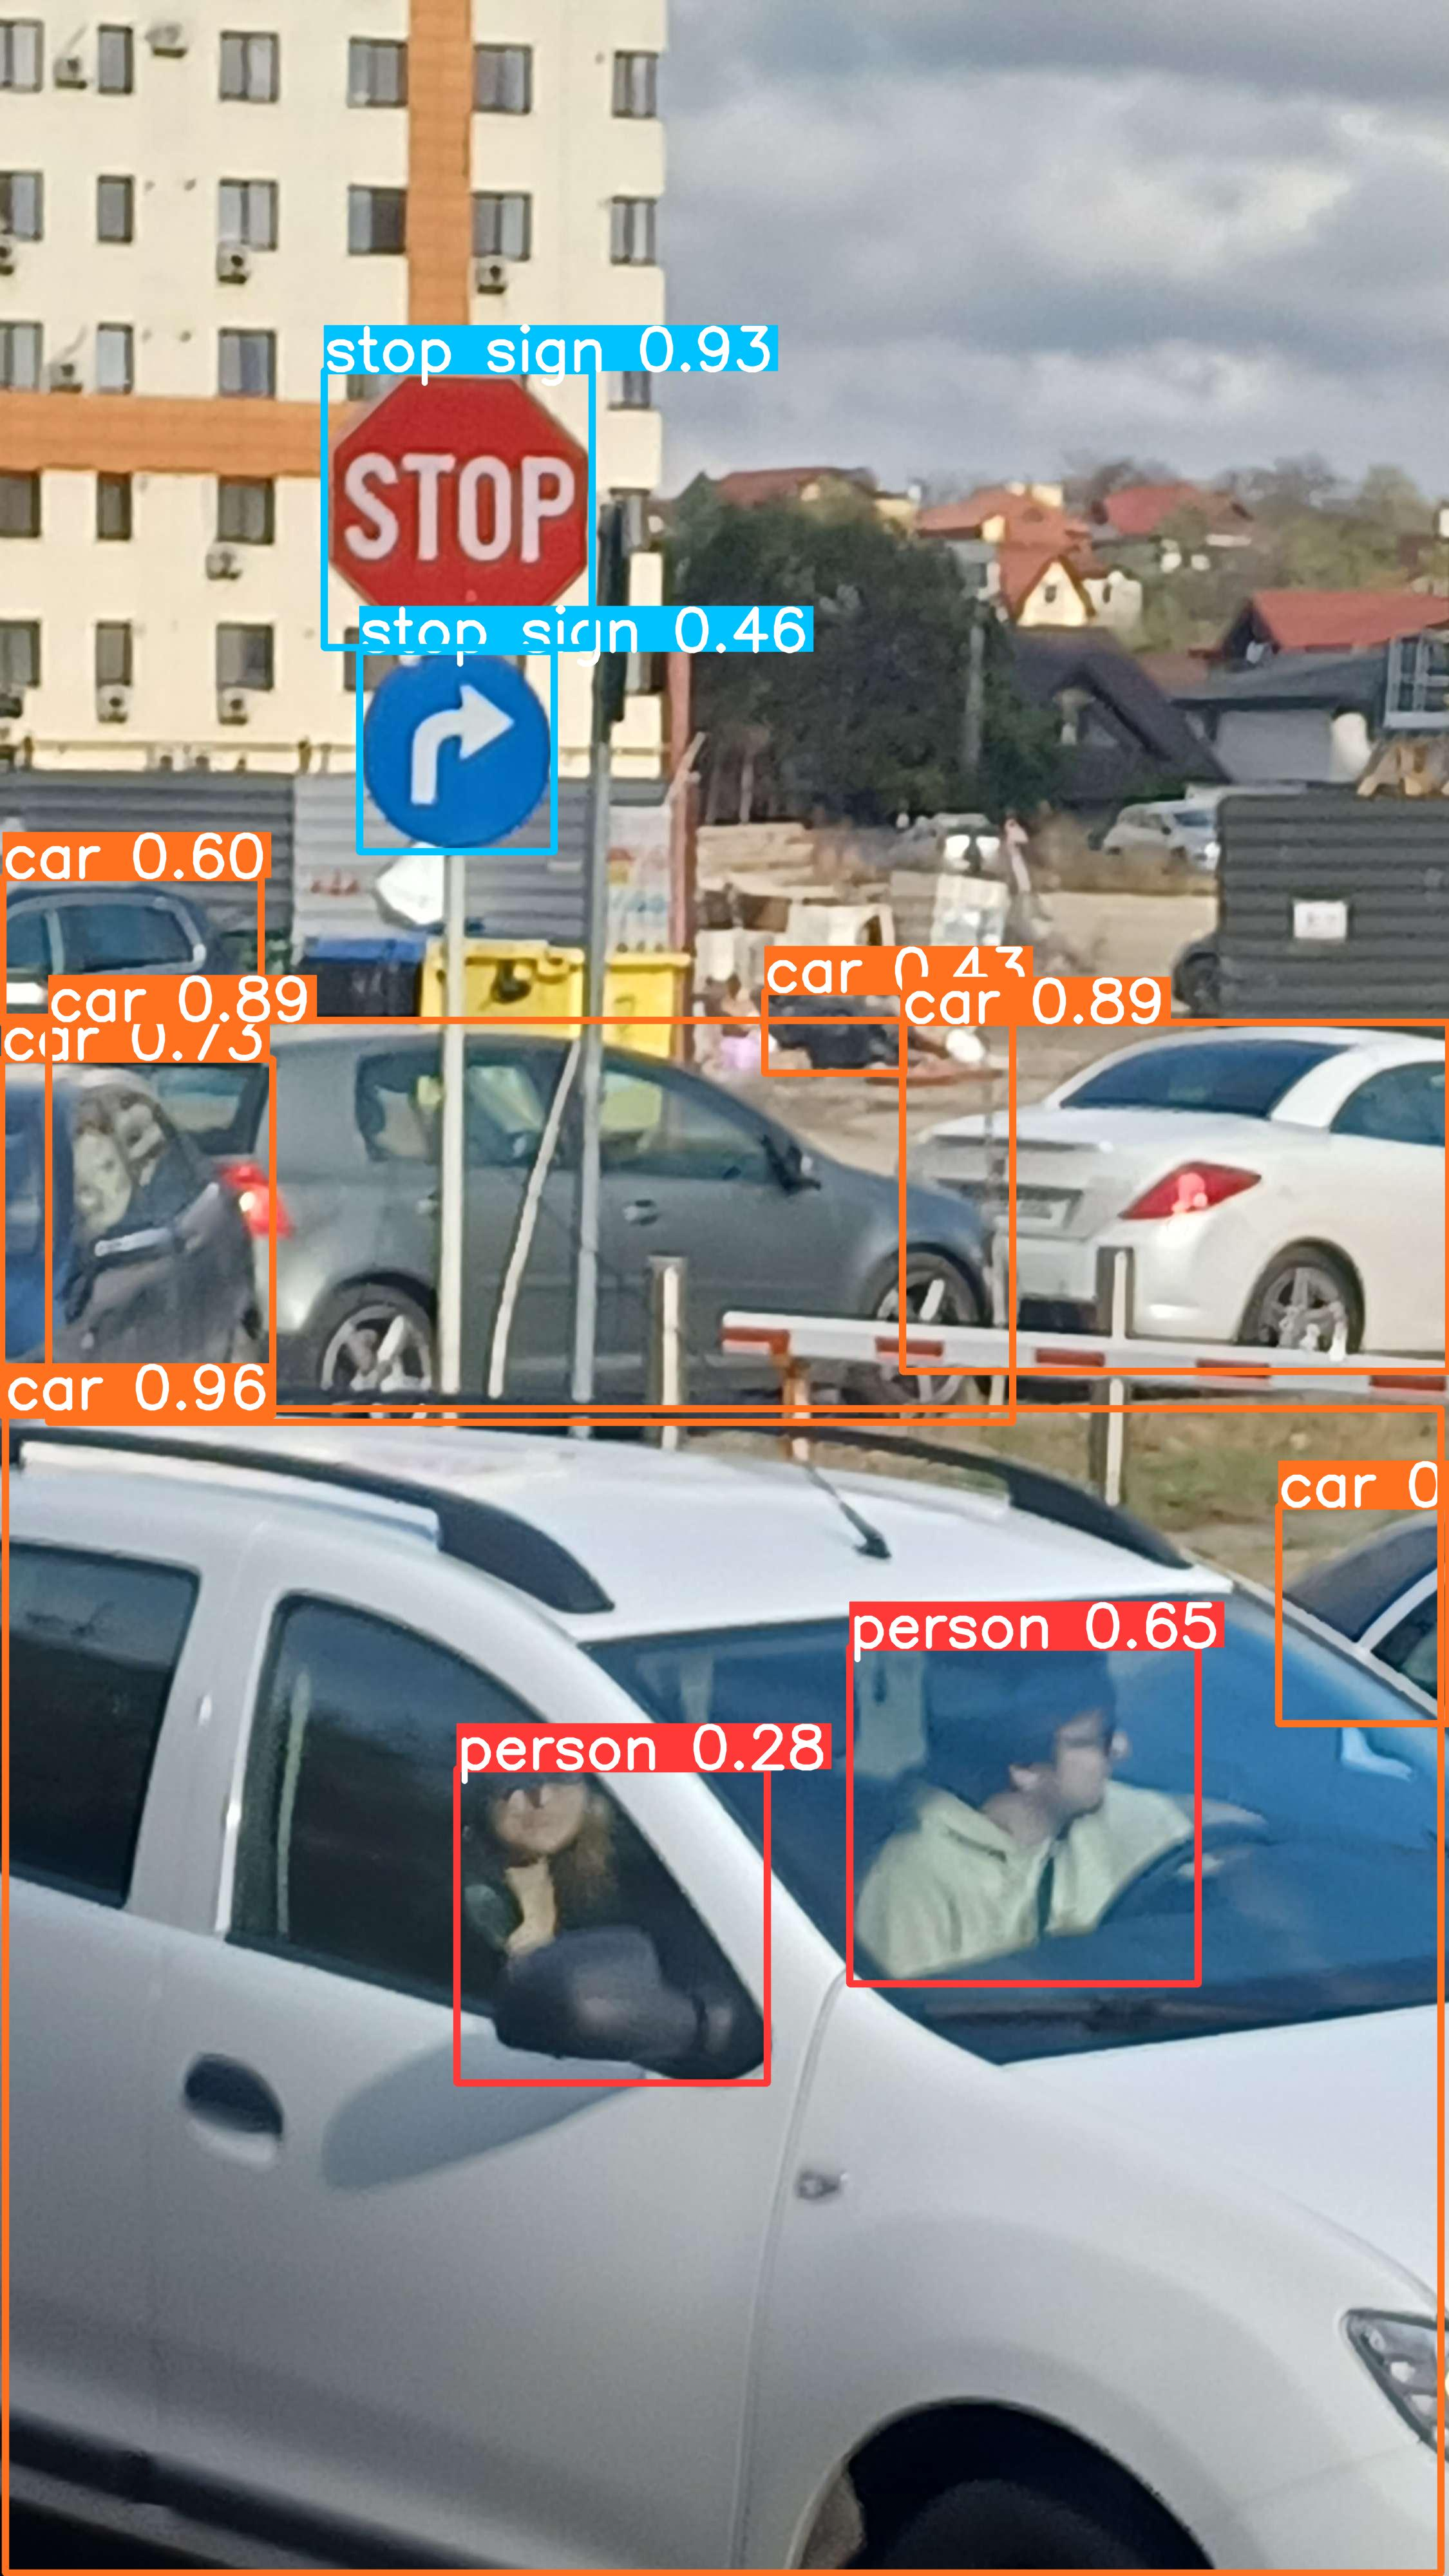
\includegraphics[width=0.5\linewidth]{poza-fata-ac-results}}
    \caption{Figure \ref{poza-fata-ac} with labels, as can be seen, the "must go right" sign is
    misclassified as a "stop sign"}
\end{figure}

\subsubsection{Roboflow}

Roboflow\footnote{Roboflow can be accessed at \url{https://roboflow.com/}} is a freemium service that provided us with two important services:
\begin{itemize}
    \item a dataset service that allows one to annotate datasets and also allows conversions
     between different dataset formats used by various preexisting architectures
    \item a model preview service, in which Roboflow will use your dataset to train a model that
    you can try in your browser --- this service can be used a maximum of 3 times per project for free
\end{itemize}

However the freemium nature of the service is a disadvantage as one might invest a lot of time in
this service due to its apparent free nature and latter be forced to buy-in when that might not have
been the original intention.

We also noticed that there was considerable delay in using the models in one's browser, we are however
not sure if this is a limitation of the models trained by Roboflow, the hardware on which they run, or
the nature of the internet connection to it.

\begin{figure*}
    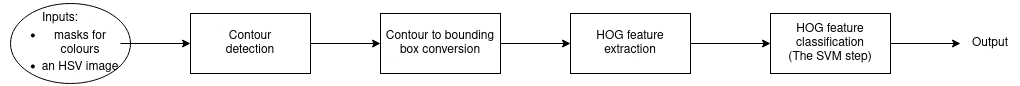
\includegraphics[width=\linewidth,]{Detection-Block-Diagram}
    \centering
    \caption{Block diagram for the SVM-based detection step}
    \noindent\rule{\textwidth}{1pt}
\end{figure*}

\section{Method description}

We propose an approach in which the process is split in two steps: a detection step and a
classification step, following existing practices in literature.

The detection step takes in an image, detects possible objects in the image that might be
road-signs (based on color, shape, etc.). The classification step takes in an image containing
only a possible road-sign and classifies it into the kind of road sign it is, or classifies it
as a non-road-sign if the detection step misdetected an object as a road-sign. These steps are
chained together using a middle layer that does any needed preprocessing on the segments from
the original image given by the detection step, and then feeds them to the classification step.

\begin{figure*}
    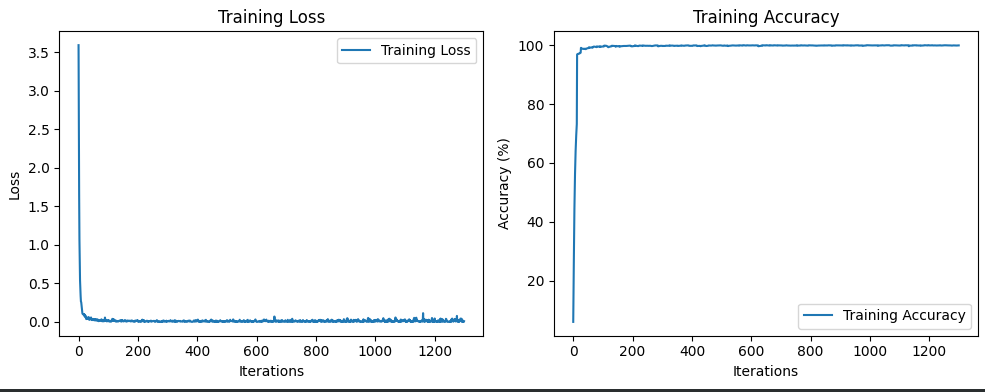
\includegraphics[width=\linewidth,]{overfit}
    \centering
    \label{img:training}
    \caption{Plot of the PyTorch-based classification training progress showing a surprisingly rapid increase in accuracy}
    \noindent\rule{\textwidth}{1pt}
\end{figure*}

\subsection{The detection step}

We've explored three approaches to detection in our work on this paper: a YOLOv8-based approach,
a fully classical approach and the SVM-based approach described in \cite{svm_paper}.

\subsubsection*{The YOLOv8-based approach}
We've chosen a neural-network-based approach for our detection step in order to see the
what differences would arrise from existing approaches taken in literature, but also in
part due to perceived ease of development\footnote{Reality often differs from one's
expectations.}.

We've decided to use a model based on the YOLOv8 architecture that we've trained on various
datasets, but have yet to find any success. Next we will explore a more classical approach
to, hopefully, obtain more success in the detection step.


\subsubsection*{The purely classical approach}
Our work on the classical approach was not a great success and did not yield great results.
This was likely due to misuse of the tools we used and incomplete understanding.

\subsubsection*{The SVM-based approach}
We generated HOG features for the images offered by the German Traffic Sign Recognition
Benchmark (GTSRB)\cite{Houben-IJCNN-2013} and trained an SVM, specifically one using a Linear
Support Vector Classification algorithm, using facilities provided by scikit-learn\cite{scikit-learn}.

\subsection{The classification step}

We explored two approaches to CNN-based\footnote{Convolutional Neural Network} classification: one was based on PyTorch\cite{Paszke_PyTorch_An_Imperative_2019}
and one was based on Keras\cite{chollet2015keras}. We used the GTSRB dataset for both approaches,
as we believe it to be high quality.

\begin{figure}[H]
    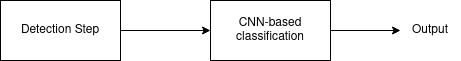
\includegraphics[width=\linewidth]{Classification-Diagram}
    \caption{Block diagram that applies to both our CNN-based approaches}
\end{figure}

\subsubsection{PyTorch}
The GTSRB dataset resembles the CIFAR10\footnote{More information at \url{https://www.cs.toronto.edu/~kriz/cifar.html}}
dataset so all we had to do is take an existing network that worked well on CIFAR10
and tweak it to work for our dataset. For training we used PyTorch\cite{Paszke_PyTorch_An_Imperative_2019} and got over
94\% accuracy on the test set. Unfortunately we highly suspect that our implementation
was heavily overfitted on our training set, and as such became unable to recognize traffic signs
in new images.

\subsubsection{Keras}
Our Keras-based CNN is a self-made implementation of the one mentioned in \cite{svm_paper}, and as such
it uses the same layers:
\begin{table}[H]
    \begin{tcolorbox}[arc=0pt,boxrule=0pt]
        \begin{tabularx}{\linewidth}{lllP{0.3\textwidth}}
            \toprule
            \thead{} & \thead{Layer} & \thead{Output Size} & \thead{Parameters} \\
            \midrule\\
            1  & Input             & $56 \times 56$ & --- \\
            2  & Convolution       & $ 96 \times 52 \times 52$ & kernel $ = 5 \times 5 $; strides $ = 1 \times 1$\\
            3  & Max Pooling       & $ 96 \times 26 \times 26$ & kernel $ = 2 \times 2 $; stride $ = 2 \times 2 $\\
            4  & Convolution       & $140 \times 24 \times 24$ & kernel $ = 3 \times 3$; strides $ = 1 \times 1$ \\
            5  & Max Pooling       & $140 \times 12 \times 12$ & kernel $ = 2 \times 2 $; stride $ = 2 \times 2$ \\
            6  & Convolution       & $240 \times 10 \times 10$ & kernel $ = 3 \times 3$; strides $ = 1 \times 1$ \\
            7  & Max Pooling       & $240 \times  5 \times  5$ & kernel $ = 2 \times 2 $; stride $ = 2 \times 2$ \\
            8  & Flatten           & $6000$ & --- \\
            9  & Densely-connected\footnote{Called "Fully connected" in the paper} & $150$ & --- \\
            10 & Dropout           & $150$  & --- \\
            11 & Densely-connected & $43$   & --- \\
            \bottomrule
        \end{tabularx}
    \end{tcolorbox}
\end{table}

The ReLU\footnote{Rectified Linear Unit activation function} layers from the original papers are missing,
as they're merged with the Convolution layers in our Keras implementation. The LRN\footnote{Local Response Normalization}
layers are missing as they are not built-in to Keras and we decided to not reimplement LRN ourselves. The
softmax layer from the original paper is part of the densely-connected layer.

\section{Results}

When we tested the approach that made use of a PyTorch-based CNN, we got over 94\% classification accuracy, and aproximately 80\%
on segmentation but it perfomed badly on our personal test, that being showing a video of
a car driving in town, or no detections on \ref{poza-fata-ac}. The training results can be seen in figure \ref{img:training}.

\section{Conclusions}

Neural-network-based approaches are very accessible --- \emph{in theory} --- but getting good
results out of them is difficult due to not being aware of mistakes that can lead to overfitting
or due to the powerful hardware needed for model training.

However, we do believe that real-time recognition of traffic signs becomes a more achievable goal
as more and more time is passing due to this high accessibility, to people who are more experienced
in the domain than us, and powerful hardware becoming more cheap with time.

\section*{APPENDIX A}\label{appendixa}
\blockcquote[Support Vector Machine (SVM) Explained - MATLAB \& Simulink]{matlabsvm}{
A support vector machine (SVM) is a supervised learning algorithm used for many classification and regression problems, including signal processing  medical applications, natural language processing, and speech and image recognition.

The objective of the SVM algorithm is to find a hyperplane that, to the best degree possible, separates data points of one class from those of another class. “Best” is defined as the hyperplane with the largest margin between the two classes, represented by plus versus minus in the figure below. Margin means the maximal width of the slab parallel to the hyperplane that has no interior data points. Only for linearly separable problems can the algorithm find such a hyperplane, for most practical problems the algorithm maximizes the soft margin allowing a small number of misclassifications.
}

As the quoted article says, SVMs are binary classifiers. It is possible to create more complex
classifiers by chaining SVMs, i.e. if SVM 1 can classify circles, and SVM 2 can classify triangles,
one can build a classifier that classifies both circles and triangles, by feeding the inputs classified
as "not circles" by SVM 1 to SVM 2.
\bibliographystyle{IEEEtran}
\bibliography{IEEEabrv,refs}
\end{document}
